\subsubsection{03.02.2016}
\textit{\textbf{Time frame:}} 19:00-21:30 

The mechanism for grasping the hurdle was improved so as to reduce the backlash of the hooks. There were put two pieces of foam rubber which kept hooks in central positions (figure \ref{Hooks1.9}). However, each hook still had some free space for movement (due to softness of foam rubber), which prevented the mechanism from brakes.

\begin{figure}[H]
	\begin{minipage}[h]{1\linewidth}
		\center{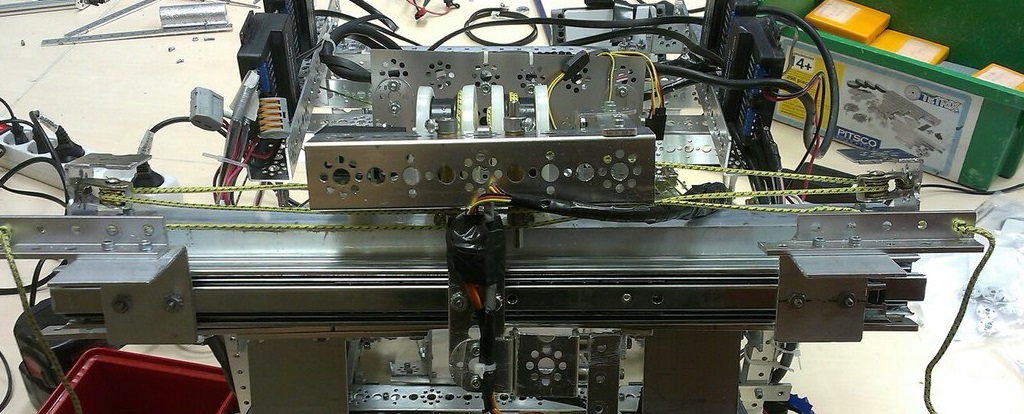
\includegraphics[scale=0.2]{3Engineering/5Team_meetings/days_of_meetings/2016.02.03/images/01}}
		\caption{Foam rubber in mechanism for grasping the hurdle}
		\label{Hooks1.9}
	\end{minipage}
\end{figure}

It was recreated the mount for the bucket. It was made according to the new principle of mounting the bucket, which included fixing the servo on the bucket, not on the mount for bucket. 

There was installed the cover for bucket (figure \ref{Bucket2.3}, \ref{Bucket2.4}).

\begin{figure}[H]
	\begin{minipage}[h]{0.47\linewidth}
		\center{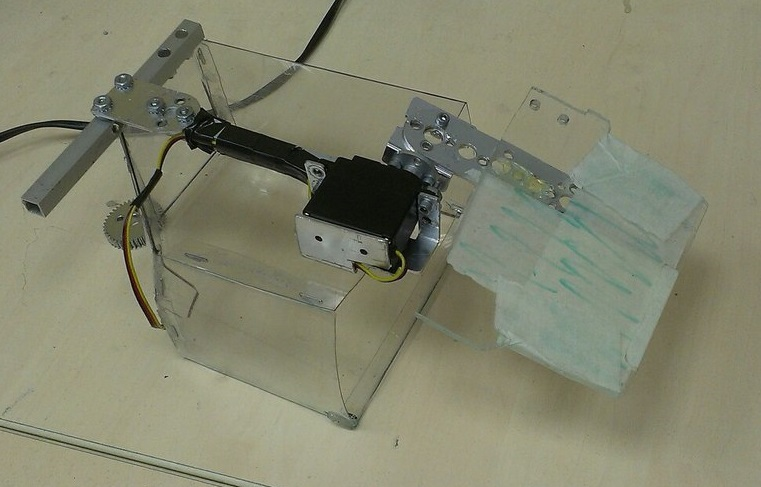
\includegraphics[scale=0.3]{3Engineering/5Team_meetings/days_of_meetings/2016.02.03/images/02}}
		\caption{Cover for bucket (opened)}
		\label{Bucket2.3}
	\end{minipage}
	\hfill
	\begin{minipage}[h]{0.47\linewidth}
		\center{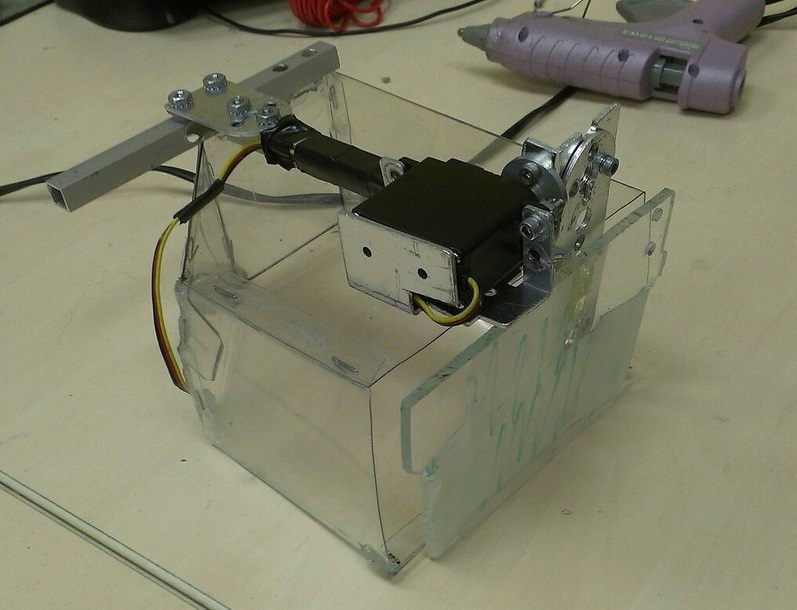
\includegraphics[scale=0.25]{3Engineering/5Team_meetings/days_of_meetings/2016.02.03/images/03}}
		\caption{Cover for bucket (closed)}
		\label{Bucket2.4}
	\end{minipage}
\end{figure}